\documentclass[11pt]{article}
\usepackage[margin=1in]{geometry}
\usepackage[expansion=false]{microtype}
\usepackage{graphicx}
\usepackage{booktabs}
\usepackage{amsmath}
\usepackage{caption}
\usepackage{float}
\usepackage[hidelinks]{hyperref}
\usepackage{enumitem}
\setlist{itemsep=2pt, topsep=4pt}
\captionsetup{font=small, labelfont=bf}
\setlength{\parindent}{0pt}
\setlength{\parskip}{6pt}

\title{Weekly Report 10/13-10/20}
\author{}
\date{}

\begin{document}
\begingroup\makeatletter\renewcommand{\@maketitle}{\begin{center}{\LARGE\@title\par}\end{center}\vspace{-4pt}}\makeatother\maketitle\endgroup

\section*{Summary}
\begin{itemize}
  \item Question: are electrodes farther from primary auditory cortex (A1) best matched by deeper layers of the frozen SpikeSpeechBrain model?
  \item Answer: yes, in all three gamma bands. Among significantly predicted electrodes, distance from A1 and best layer are positively rank-correlated (Spearman $\rho$, 95\% subject-bootstrap CI):
  \begin{itemize}
    \item High gamma: $0.57$ (0.43 to 0.70), $n = 199$
    \item Mid gamma: $0.48$ (0.36 to 0.56), $n = 260$
    \item Low gamma: $0.43$ (0.32 to 0.52), $n = 191$
  \end{itemize}
  \item Within-subject permutation test: $p < 0.0001$ in each band.
  \item Regressing the audio envelope out of the ECoG leaves high gamma unchanged: $\rho = 0.58$, $n = 156$.
  \item Correction to last week: the audio-envelope dry run is $\rho = -0.327$ once bands are built from the dataset's preprocessed signal (earlier $-0.205$ came from raw EDF bands without notch filtering, common average reference or spike removal).
  \item Model activations come from a placeholder inference run, so results are provisional.
\end{itemize}

\section{Data and preprocessing}
\begin{itemize}
  \item \textbf{ECoG:} Podcast ECoG dataset (OpenNeuro ds005574), 9 subjects listening to a 30-minute episode of \emph{This American Life} (more than 5,000 words, about 10 speakers).
  \begin{itemize}
    \item 1,330 electrodes in the dataset; I analyze the 1,268 in \texttt{electrodes\_good\_labeled.csv}.
    \item Each electrode has a distance to the A1 centroid and an anatomical parcel and stage label.
  \end{itemize}
  \item \textbf{Dataset preprocessing} (\texttt{ecogprep}, per the dataset paper): 512 Hz sampling, bad electrodes flagged from power spectra, outlier time points removed and interpolated, common average reference, notch filters at 60, 120, 180 and 240 Hz. I start from the unfiltered \texttt{ecogprep} files.
  \item \textbf{Bands:} 4th-order zero-phase Butterworth band-pass, Hilbert envelope, 80 ms mean bins (22,500 frames), z-score per electrode.
  \begin{itemize}
    \item Low gamma 30 to 60 Hz, mid gamma 60 to 90 Hz, high gamma 90 to 150 Hz.
    \item Theta (4 to 8 Hz) and beta (13 to 30 Hz) are exported and not yet analyzed.
  \end{itemize}
  \item \textbf{Model activations:} frozen SpikeSpeechBrain (trained on LibriSpeech), run by Pavlos on the podcast audio in 30 s windows with 4 s padding (placeholder).
  \begin{itemize}
    \item 15 layers, 1,024 channels each, from the memory state (\texttt{mems}).
    \item Segments are placed at their start time on the 80 ms clock and overlapping frames are averaged, covering 94.9\% of frames.
  \end{itemize}
  \item \textbf{Speaker labels:} pyannote diarization on the audio, aligned to word timings and sent to Pavlos for the next inference run. Not used in any analysis here.
\end{itemize}

\section{Methods}
\subsection{Envelope dry run}
\begin{itemize}
  \item Audio averaged to mono, band-passed 100 Hz to $\min(8\,\mathrm{kHz}, 0.45\,f_s)$, Hilbert amplitude, 80 ms bins.
  \item For each electrode: correlate the 90 to 150 Hz signal with the envelope at lags $-400$ to $+960$ ms and keep the peak Pearson $r$.
  \item Spearman correlation between distance from A1 and peak $r$ across electrodes.
\end{itemize}

\subsection{Gate 1: feature-based similarity}
For each layer and electrode:
\begin{enumerate}
  \item \textbf{Features:} 1,024 channels reduced to 64 principal components (unit variance), with 8 lags (0 to 560 ms), giving 512 predictors per frame. 14,406 of 22,500 frames are usable.
  \item \textbf{Cross-validation:} 5 contiguous blocks, with 25 frames on either side of the test block removed from training.
  \item \textbf{Ridge regression:} $w = (X^\top X + \alpha I)^{-1} X^\top y$, fit on training frames only, $\alpha$ from $10^3$ to $10^7$ chosen per layer by mean held-out correlation.
  \item \textbf{Score:} Pearson correlation between predicted and recorded signal on the test block, averaged over folds.
\end{enumerate}
\begin{itemize}
  \item Repeated for all 15 layers; an electrode's best layer is the one with the highest score.
  \item The model is the only predictor: electrodes are not compared with each other.
\end{itemize}

\subsection{Significance filter}
\begin{itemize}
  \item Circularly shift each ECoG signal by a random offset of at least 60 s, refit all 15 layers, keep the best score. Repeated 20 times and pooled per band.
  \item An electrode is significant if its real best score exceeds the null at $p < 0.01$.
  \item Cutoffs: $r = 0.079$ (low gamma), $0.082$ (mid gamma), $0.125$ (high gamma).
\end{itemize}

\subsection{Statistics}
\begin{itemize}
  \item \textbf{Spearman $\rho$:} distance from A1 against best layer, among significant electrodes.
  \item \textbf{Subject bootstrap:} resample subjects with replacement 2,000 times; the 2.5th and 97.5th percentiles give the 95\% CI.
  \item \textbf{Slope:} ordinary least-squares slope of best layer on distance (layers per 10 mm), among significant electrodes. Its $p$-values come from the same two tests: a subject bootstrap (10,000 resamples; two-sided $p$ is twice the smaller tail fraction) and a within-subject permutation of best-layer labels (10,000 shuffles).
  \item \textbf{Band comparison:} the same bootstrap resample of subjects is applied to all three bands, and the difference in $\rho$ or slope between two bands is computed for each resample (paired). The 2.5th and 97.5th percentiles give the CI of the difference.
  \item \textbf{Within-subject permutation:} shuffle best-layer labels among each subject's significant electrodes 10,000 times; $p = (1 + k)/10{,}001$, so the smallest possible value is $0.0001$. A global shuffle ignoring subjects was also run.
\end{itemize}

\subsection{Controls and breakdowns}
\begin{itemize}
  \item \textbf{Envelope regression:} regress lagged audio envelope (0 to 960 ms, 13 lags) and an intercept out of each electrode, then rerun the full pipeline including the significance filter.
  \item \textbf{Ridge grid:} high gamma rerun with $\alpha$ from $10^5$ to $10^9$.
  \item \textbf{Brain areas:} best layers of significant electrodes grouped by parcel, ordered by median distance from A1.
\end{itemize}

\section{Results}
\subsection{Audio-envelope dry run}
\begin{itemize}
  \item Electrodes closer to A1 track the audio envelope more strongly (Table~\ref{tab:dry}, Figure~\ref{fig:dry}).
  \item With preprocessed signal, my 90 to 150 Hz band and the dataset's 70 to 200 Hz high gamma give the same correlation ($-0.327$ and $-0.325$).
  \item Raw-EDF bands gave $-0.205$: the earlier difference came from preprocessing, not band width.
  \item For the top 10\% of electrodes, the median peak lag is 80 ms and every peak falls between 0 and 640 ms, so the brain signal follows the audio.
\end{itemize}

\begin{table}[H]
\centering\small\setlength{\tabcolsep}{4pt}
\caption{Spearman correlation between distance from A1 and peak envelope correlation. CI is the 95\% subject-bootstrap interval. Permutation $p$ uses 5,000 within-subject shuffles.}
\label{tab:dry}
\begin{tabular}{lcccc}
\toprule
ECoG signal & $n$ & $\rho$ & 95\% CI & permutation $p$ \\
\midrule
My band, 90--150 Hz, from preprocessed \texttt{ecogprep} & 1268 & $-0.327$ & $-0.44$ to $-0.24$ & $<0.0002$ \\
Dataset high gamma, 70--200 Hz & 1268 & $-0.325$ & $-0.44$ to $-0.23$ & $<0.0002$ \\
My band, 90--150 Hz, from raw EDF (superseded) & 1268 & $-0.205$ & $-0.33$ to $-0.10$ & $<0.0002$ \\
\midrule
My band, preprocessed, stages 1--5 only & 385 & $-0.353$ & $-0.58$ to $-0.11$ & $<0.0002$ \\
Dataset high gamma, stages 1--5 only & 385 & $-0.338$ & $-0.57$ to $-0.08$ & $<0.0002$ \\
\bottomrule
\end{tabular}
\end{table}

\IfFileExists{figures/envelope_dry_run.png}{%
\begin{figure}[H]
\centering
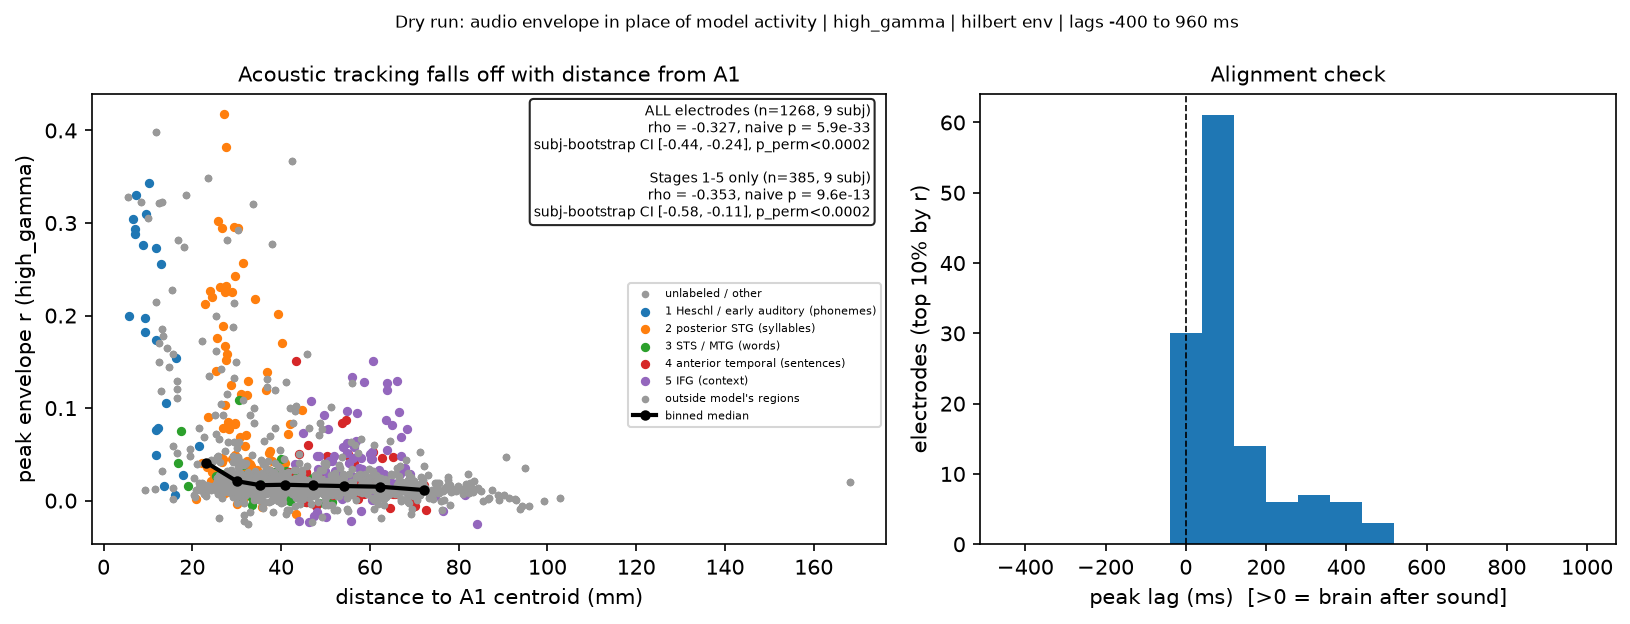
\includegraphics[width=0.95\linewidth]{figures/envelope_dry_run.png}
\caption{Audio-envelope dry run on the preprocessed 90 to 150 Hz high gamma. Left: peak envelope correlation against distance from A1 for each electrode, colored by anatomical stage, with the binned median in black and the statistics from Table~\ref{tab:dry}. Right: lag of the peak for the 10\% of electrodes with the highest correlation (positive lag means the brain signal follows the sound).}
\label{fig:dry}
\end{figure}}{}


\subsection{Gate 1 across gamma bands}
\begin{itemize}
  \item Best layer increases with distance from A1 in all three bands (Table~\ref{tab:gate1}, Figure~\ref{fig:gate1}); high gamma is strongest.
  \item Across all 1,268 electrodes, including those failing the filter, $\rho$ is much lower (0.135, 0.107, 0.140 for high, mid, low gamma), so the trend describes electrodes the model predicts.
\end{itemize}

\begin{table}[H]
\centering\small\setlength{\tabcolsep}{4pt}
\caption{Gate 1 results per band (\texttt{mems}, 15 layers, preprocessed signal). $n$ is the number of significant electrodes out of 1,268. The last column is the 95th percentile of $|\rho|$ under the within-subject shuffle.}
\label{tab:gate1}
\begin{tabular}{lccccccc}
\toprule
Band & $n$ & subjects & $\rho$ & 95\% CI & permutation $p$ & shuffle 95th pct & $\rho$ (all 1,268) \\
\midrule
High gamma & 199 & 9 & 0.57 & 0.43 to 0.70 & $<0.0001$ & 0.29 & 0.135 \\
Mid gamma  & 260 & 9 & 0.48 & 0.36 to 0.56 & $<0.0001$ & 0.20 & 0.107 \\
Low gamma  & 191 & 8 & 0.43 & 0.32 to 0.52 & $<0.0001$ & 0.20 & 0.140 \\
\bottomrule
\end{tabular}
\end{table}

\begin{figure}[H]
\centering
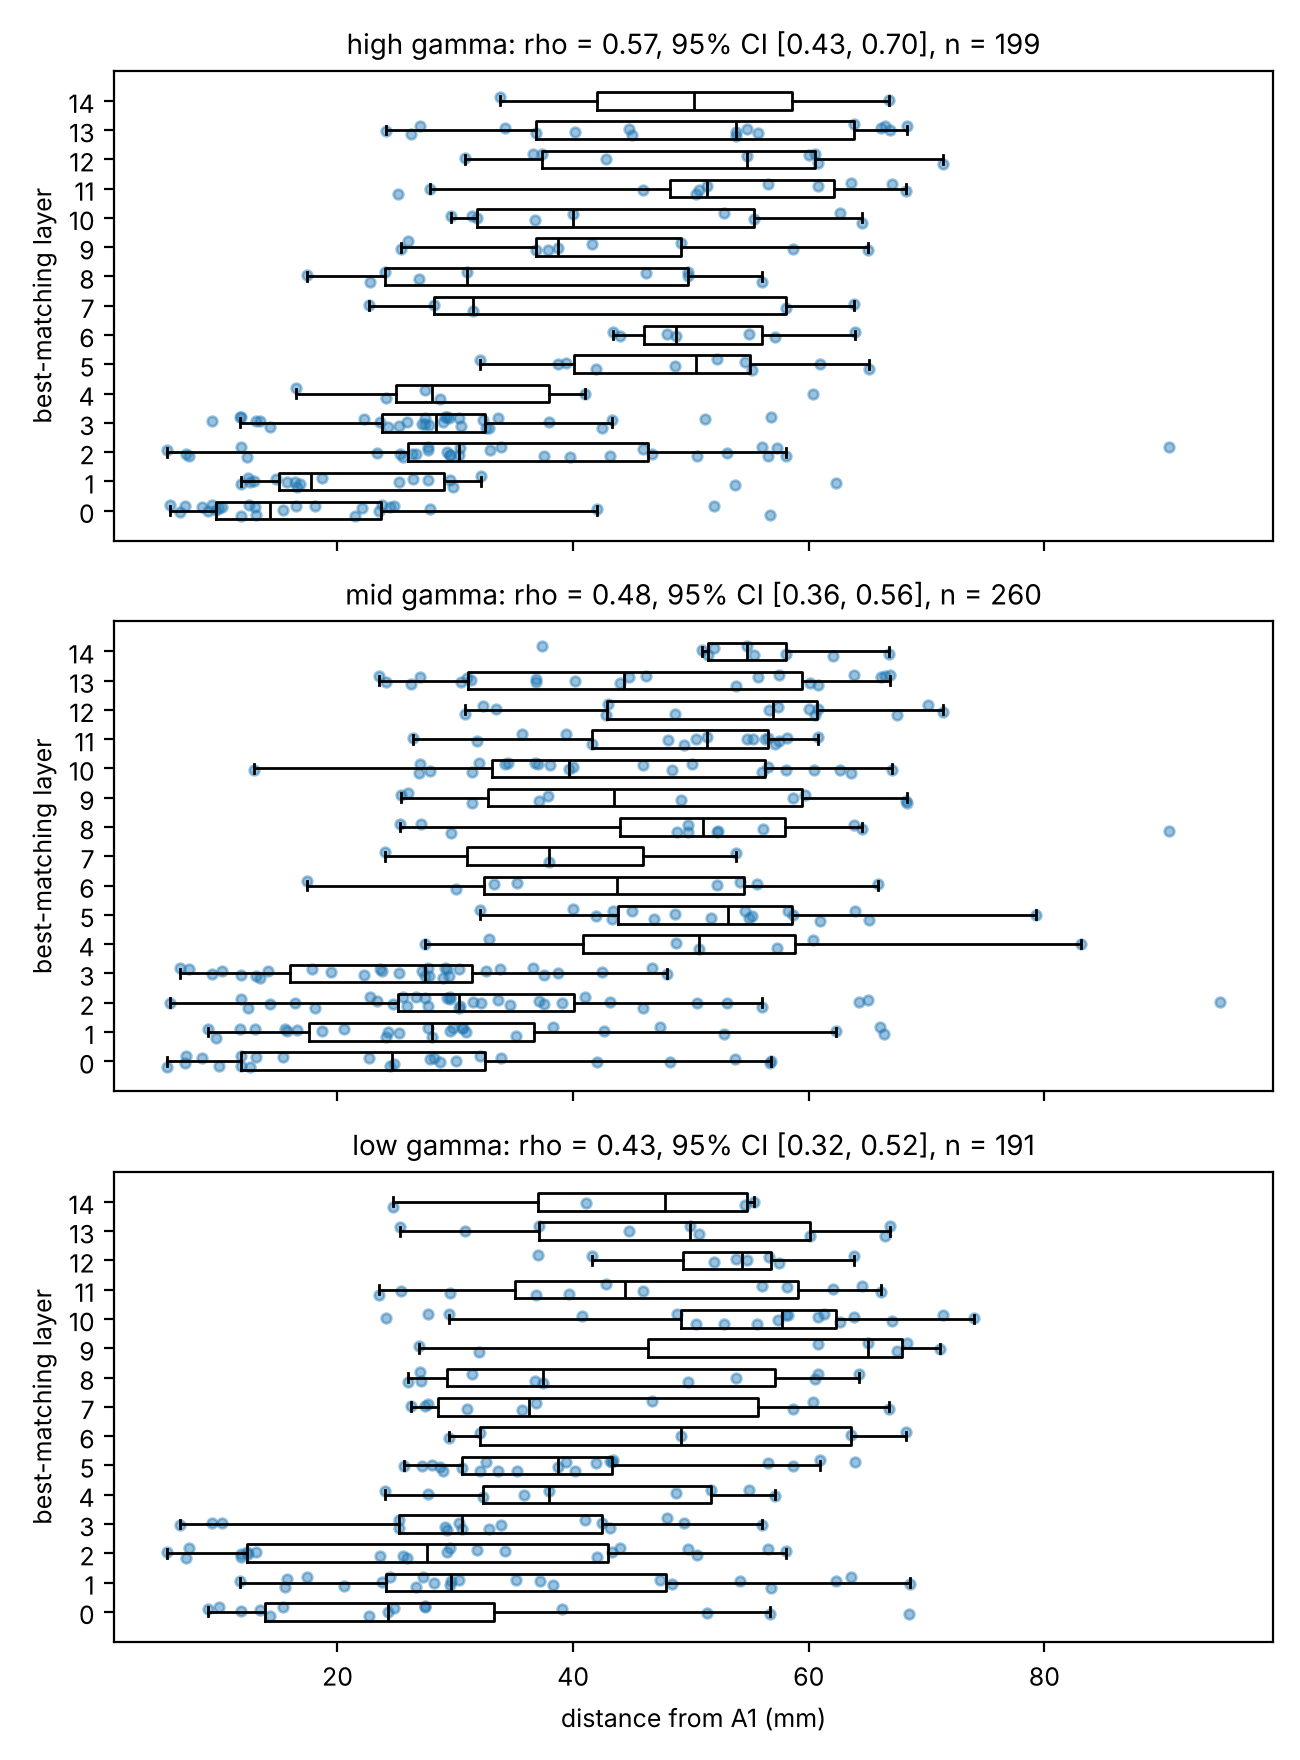
\includegraphics[width=\linewidth,height=0.88\textheight,keepaspectratio]{figures/gate1_dist_vs_layer.png}
\caption{Distance from A1 against best-matching layer for significant electrodes, one panel per band (high, mid and low gamma from top to bottom). Each dot is an electrode, and boxes show the distances of electrodes that chose each layer. Titles give $\rho$, the 95\% subject-bootstrap CI and $n$.}
\label{fig:gate1}
\end{figure}


\subsection{Permutation test}
\begin{itemize}
  \item The observed $\rho$ is above all 10,000 shuffled values in every band (Figure~\ref{fig:perm}).
  \item The shuffled distribution sits above zero because shuffling within a subject preserves between-subject differences (a subject with farther electrodes may also have deeper best layers).
  \item The gap between observed $\rho$ and the shuffled 95th percentile measures structure within subjects: 0.23 in low gamma, 0.28 in mid gamma, 0.28 in high gamma.
\end{itemize}

\begin{figure}[H]
\centering
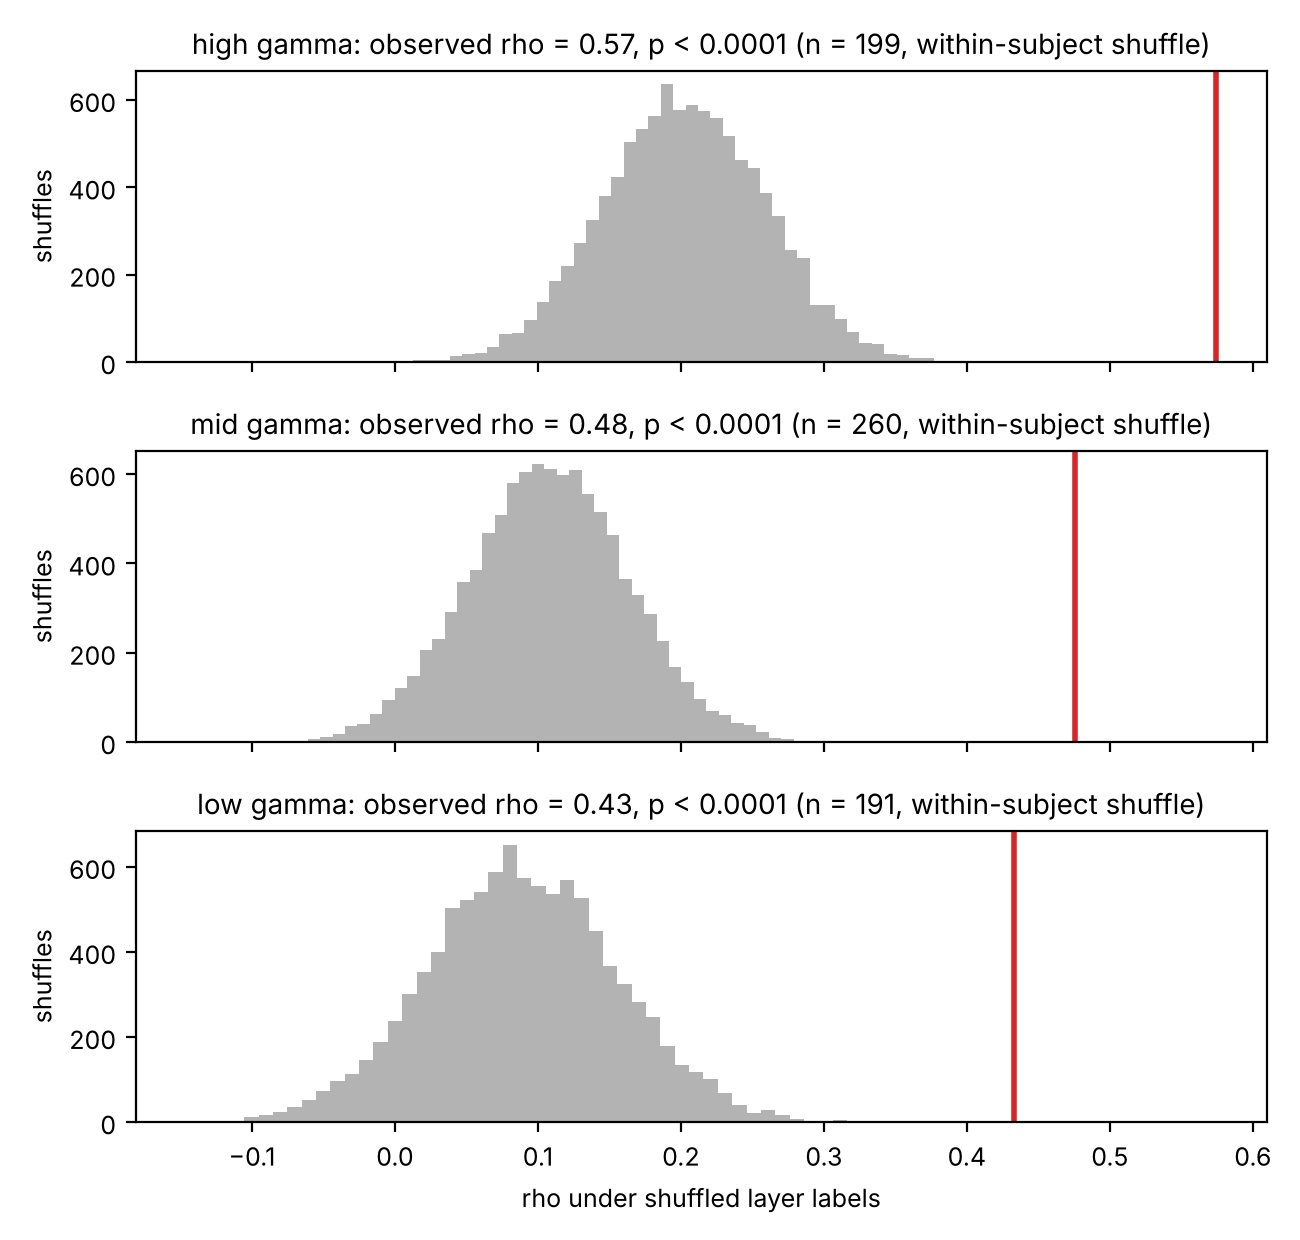
\includegraphics[width=0.95\linewidth,height=0.62\textheight,keepaspectratio]{figures/gate1_permutation.png}
\caption{Distribution of $\rho$ under 10,000 within-subject shuffles of best-layer labels (grey) and the observed $\rho$ (red line), per band (high, mid and low gamma from top to bottom).}
\label{fig:perm}
\end{figure}


\subsection{Slope and band comparison}
\begin{itemize}
  \item The regression slope of best layer on distance is positive in every band, with $p < 0.001$ under both the subject bootstrap and the within-subject permutation (Table~\ref{tab:slope}).
  \item High gamma rises 1.34 layers per 10 mm, mid gamma 1.17 and low gamma 1.09.
  \item High gamma has a higher $\rho$ than mid gamma (difference 0.10, 95\% CI 0.03 to 0.18) and than low gamma (0.14, CI 0.05 to 0.24).
  \item Mid gamma and low gamma are not separable (difference 0.04, CI $-0.05$ to 0.15).
  \item For slope, only high against mid gamma excludes zero (difference 0.17 layers per 10 mm, CI 0.01 to 0.30). High against low (0.26, CI $-0.06$ to 0.59) and mid against low (0.08, CI $-0.26$ to 0.45) do not.
  \item The ordering high $>$ mid $>$ low is therefore supported for high gamma against the other two bands in $\rho$, and not between mid and low gamma.
\end{itemize}

\begin{table}[H]
\centering\small\setlength{\tabcolsep}{4pt}
\caption{Slope of best layer on distance from A1 (layers per 10 mm) among significant electrodes. CI is the 95\% subject-bootstrap interval (10,000 resamples). The last column is the 95th percentile of the absolute slope under the within-subject shuffle. Band differences use the same paired resamples.}
\label{tab:slope}
\begin{tabular}{lcccccc}
\toprule
Band & $n$ & slope & 95\% CI & boot. $p$ & perm. $p$ & shuffle 95th \\
\midrule
High gamma & 199 & 1.34 & 0.92 to 1.58 & 0.0002 & 0.0001 & 0.70 \\
Mid gamma  & 260 & 1.17 & 0.79 to 1.44 & 0.0002 & 0.0001 & 0.54 \\
Low gamma  & 191 & 1.09 & 0.73 to 1.32 & 0.0002 & 0.0001 & 0.50 \\
\midrule
\multicolumn{7}{l}{Band differences (paired subject bootstrap)} \\
\midrule
\multicolumn{2}{l}{Comparison} & metric & difference & 95\% CI & $p$ & \\
\midrule
\multicolumn{2}{l}{High $-$ mid} & $\rho$ & 0.098 & 0.031 to 0.183 & 0.010 & \\
\multicolumn{2}{l}{High $-$ low} & $\rho$ & 0.141 & 0.046 to 0.236 & 0.004 & \\
\multicolumn{2}{l}{Mid $-$ low} & $\rho$ & 0.043 & $-0.045$ to 0.151 & 0.355 & \\
\multicolumn{2}{l}{High $-$ mid} & slope & 0.175 & 0.013 to 0.297 & 0.039 & \\
\multicolumn{2}{l}{High $-$ low} & slope & 0.258 & $-0.060$ to 0.594 & 0.098 & \\
\multicolumn{2}{l}{Mid $-$ low} & slope & 0.083 & $-0.264$ to 0.453 & 0.567 & \\
\bottomrule
\end{tabular}
\end{table}

\subsection{Acoustic control}
\begin{itemize}
  \item With the lagged envelope regressed out, high gamma gives $\rho = 0.58$ (95\% CI 0.43 to 0.69), 156 significant electrodes, against $\rho = 0.57$ and 199 electrodes without the control (Figure~\ref{fig:envreg}).
  \item The envelope explains a median of 0.1\% of an electrode's variance, at most 19.9\%.
  \item The 43 electrodes that lose significance had less envelope content (median 0.7\% against 2.5\%), were farther from A1 (38.7 mm against 30.3 mm) and had median best layer 4 against 3.
  \item This removes broadband loudness only; spectral content and syllable onsets remain.
\end{itemize}

\begin{figure}[H]
\centering
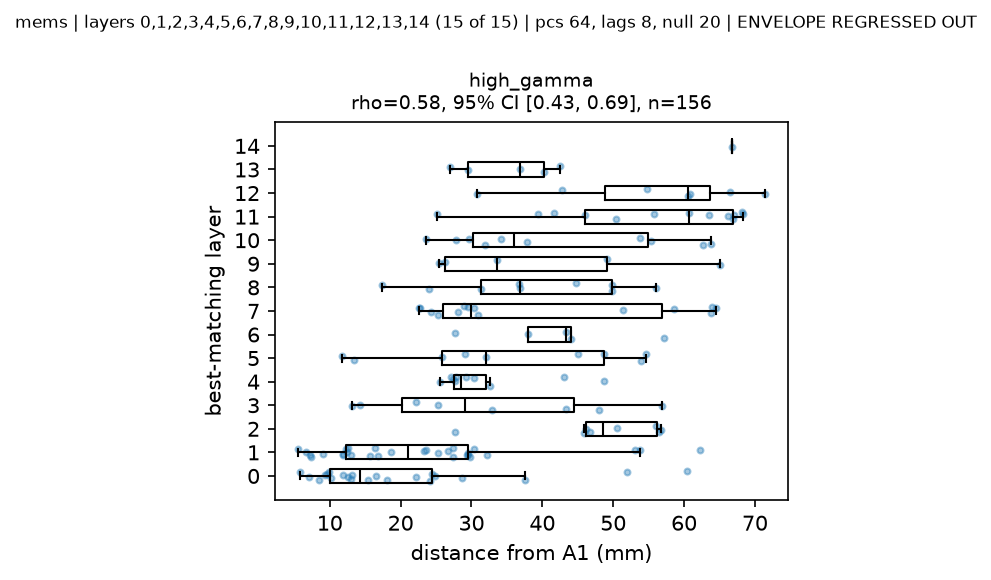
\includegraphics[width=0.95\linewidth,height=0.6\textheight,keepaspectratio]{figures/envreg_dist_vs_layer.png}
\caption{High-gamma Gate 1 with the lagged audio envelope regressed out of each electrode. Layout as in Figure~\ref{fig:gate1}.}
\label{fig:envreg}
\end{figure}


\subsection{Ridge penalty}
\begin{itemize}
  \item High gamma alone with $\alpha$ from $10^5$ to $10^9$: 195 significant electrodes, $\rho = 0.57$ (95\% CI 0.45 to 0.66), the same as the default grid.
  \item In the three-band run, one penalty per layer is shared across bands and reaches the grid edge ($10^7$) for 6 of 15 layers. With high gamma alone, the chosen penalty is $10^5$ or $10^6$ for most layers.
\end{itemize}

\subsection{Brain areas}
\begin{itemize}
  \item Closest to A1 (within 20 mm) and earliest layers: medial belt (10 electrodes, median layer 1.0), primary auditory cortex (3 electrodes, 0.0), posterior insular areas (0.0 to 1.0).
  \item Farthest (63 to 67 mm) and deepest layers: IFSa (11 electrodes, median layer 11.0), posterior 47r (4 electrodes, 13.0).
  \item Across parcels with at least 3 significant electrodes, Spearman between median distance and median layer: 0.71 in high gamma (23 parcels), 0.72 in mid gamma (28), 0.77 in low gamma (19). These are descriptive values on parcel medians.
  \item Exceptions:
  \begin{itemize}
    \item Superior temporal visual area: about 27 mm from A1, median layer 9.0 in high gamma (5 electrodes, 3 subjects), 9.5 in mid gamma, 2.0 in low gamma.
    \item Auditory 4 Complex (29 electrodes, 8 subjects): spans layers 0 to 13 at similar distances.
    \item Area 55b: 45 mm away, median layer 3.0.
  \end{itemize}
  \item Many parcels have only 1 to 3 subjects (IFSp and STGa one in high gamma), so parcel and subject effects are not separable.
\end{itemize}

\begin{figure}[p]
\centering
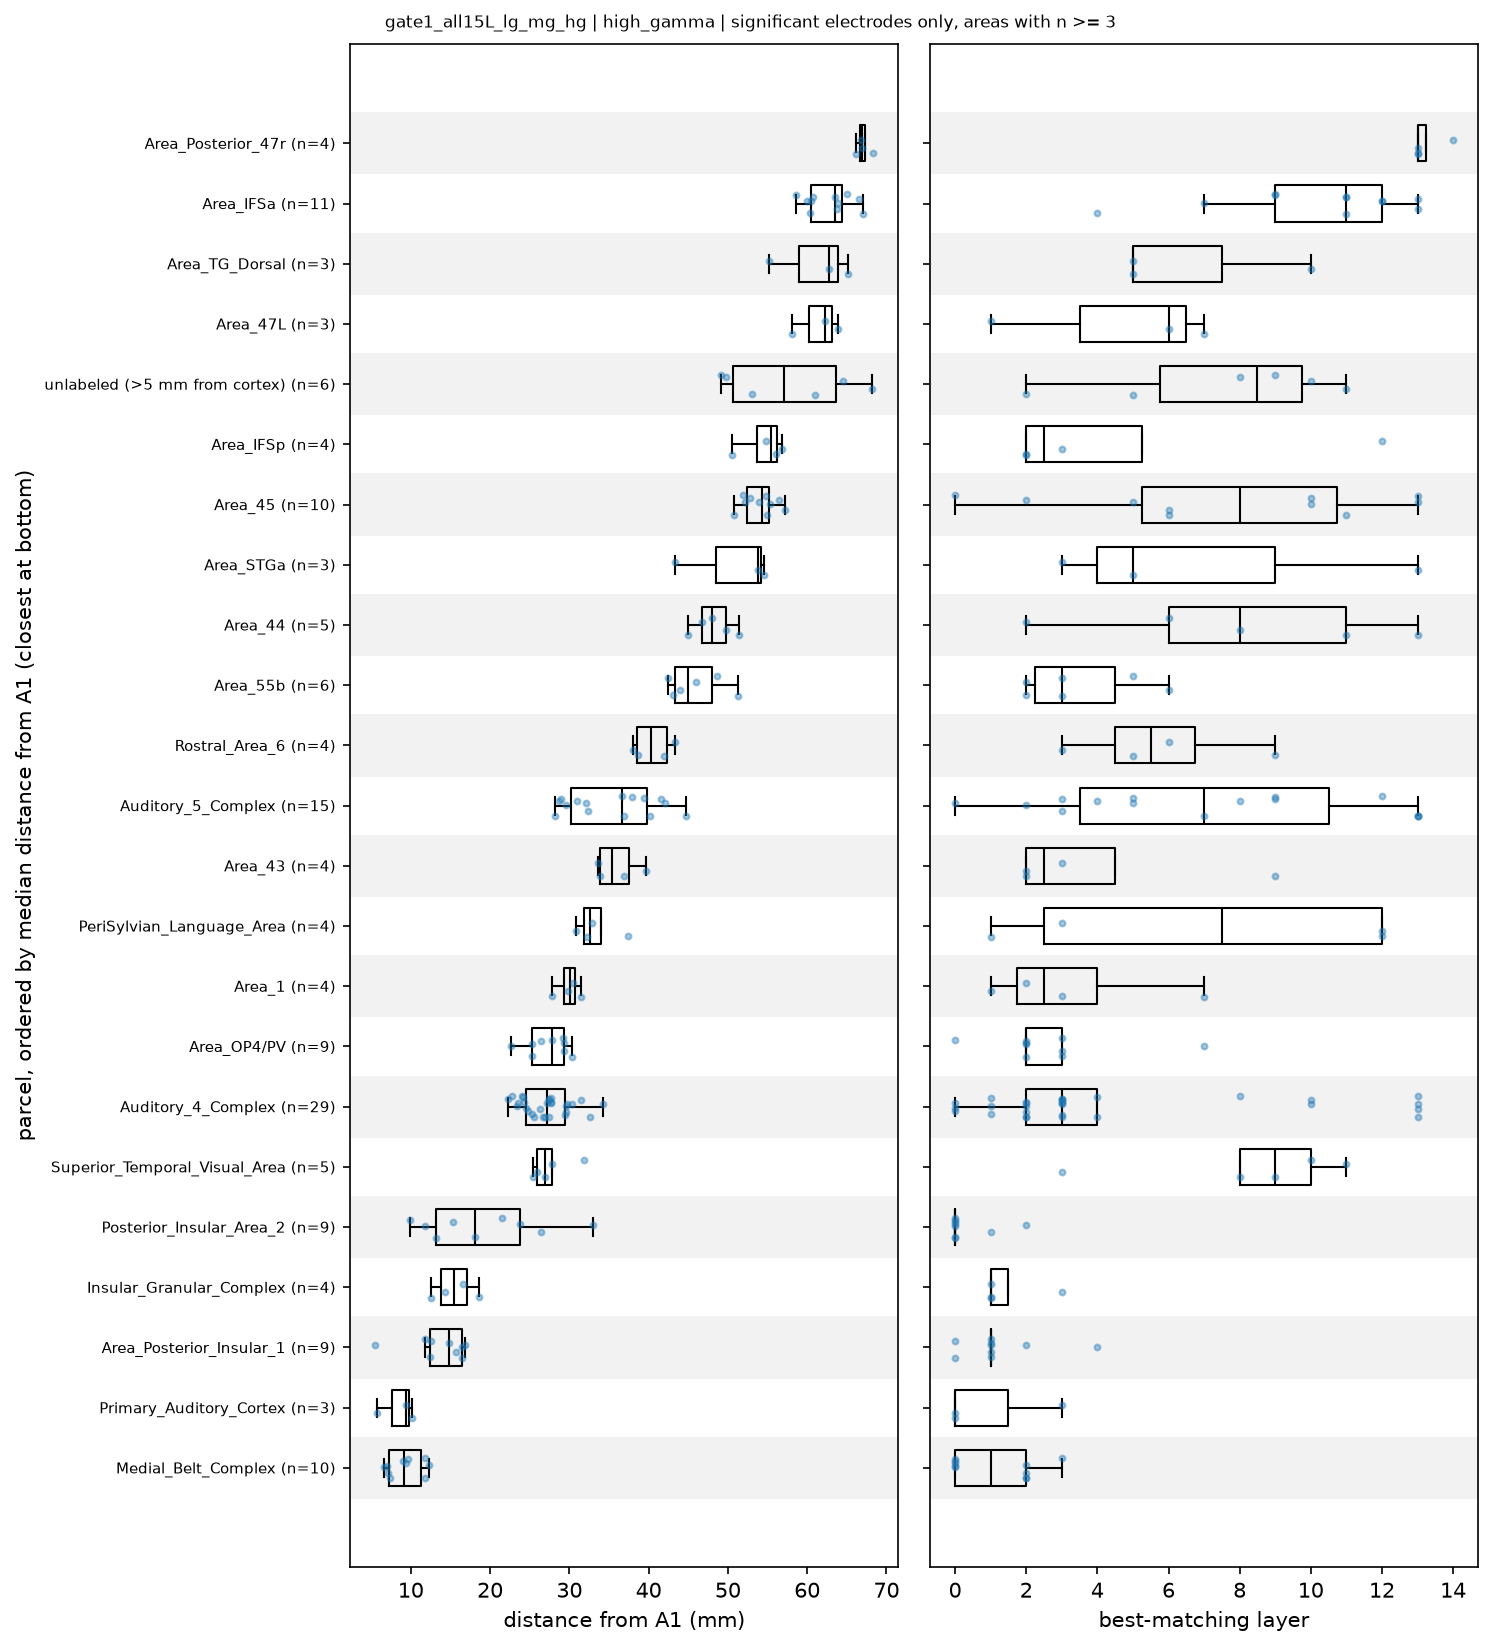
\includegraphics[width=\linewidth,height=0.82\textheight,keepaspectratio]{figures/areas_high_gamma.png}
\caption{High-gamma best-matching layer by parcel, for parcels with at least 3 significant electrodes (164 of 199 electrodes). Parcels are ordered by median distance from A1 (closest at the bottom). Left: distance from A1. Right: best-matching layer.}
\label{fig:areas}
\end{figure}



\subsection{Layer profile}
\begin{itemize}
  \item Mean held-out correlation across all electrodes peaks at layer 2 in every band and is lowest at layer 14 (Figure~\ref{fig:curves}).
  \item Absolute correlations are small because most electrodes are not predicted by any layer.
\end{itemize}

\begin{figure}[H]
\centering
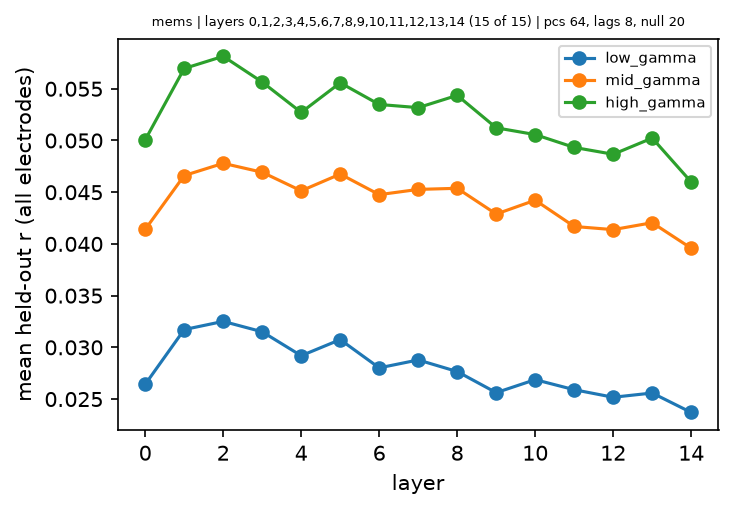
\includegraphics[width=0.62\linewidth]{figures/layer_curves.png}
\caption{Mean held-out correlation across all 1,268 electrodes for each layer and band.}
\label{fig:curves}
\end{figure}


\section{Next steps}
\begin{itemize}
  \item Literature check: Li et al. 2023 (Nature Neuroscience) reports deeper DNN layers matching higher-order auditory cortex; I will read it and the two other papers Costas shared.
  \item Analyze theta and beta, and the residual and spike arrays.
  \item Rerun after the final inference run, with speaker information from the diarization.
  \item Control with a randomly initialized copy of the model.
  \item Full-pipeline shift test on the cluster.
  \item SNN ablation or perturbation (for example removing feedback) to test its effect on the distance-to-layer relationship.
  \item Check the literature for whether a distance-to-depth gradient is expected from any hierarchical model.
\end{itemize}

\clearpage

\begin{figure}[H]
\centering
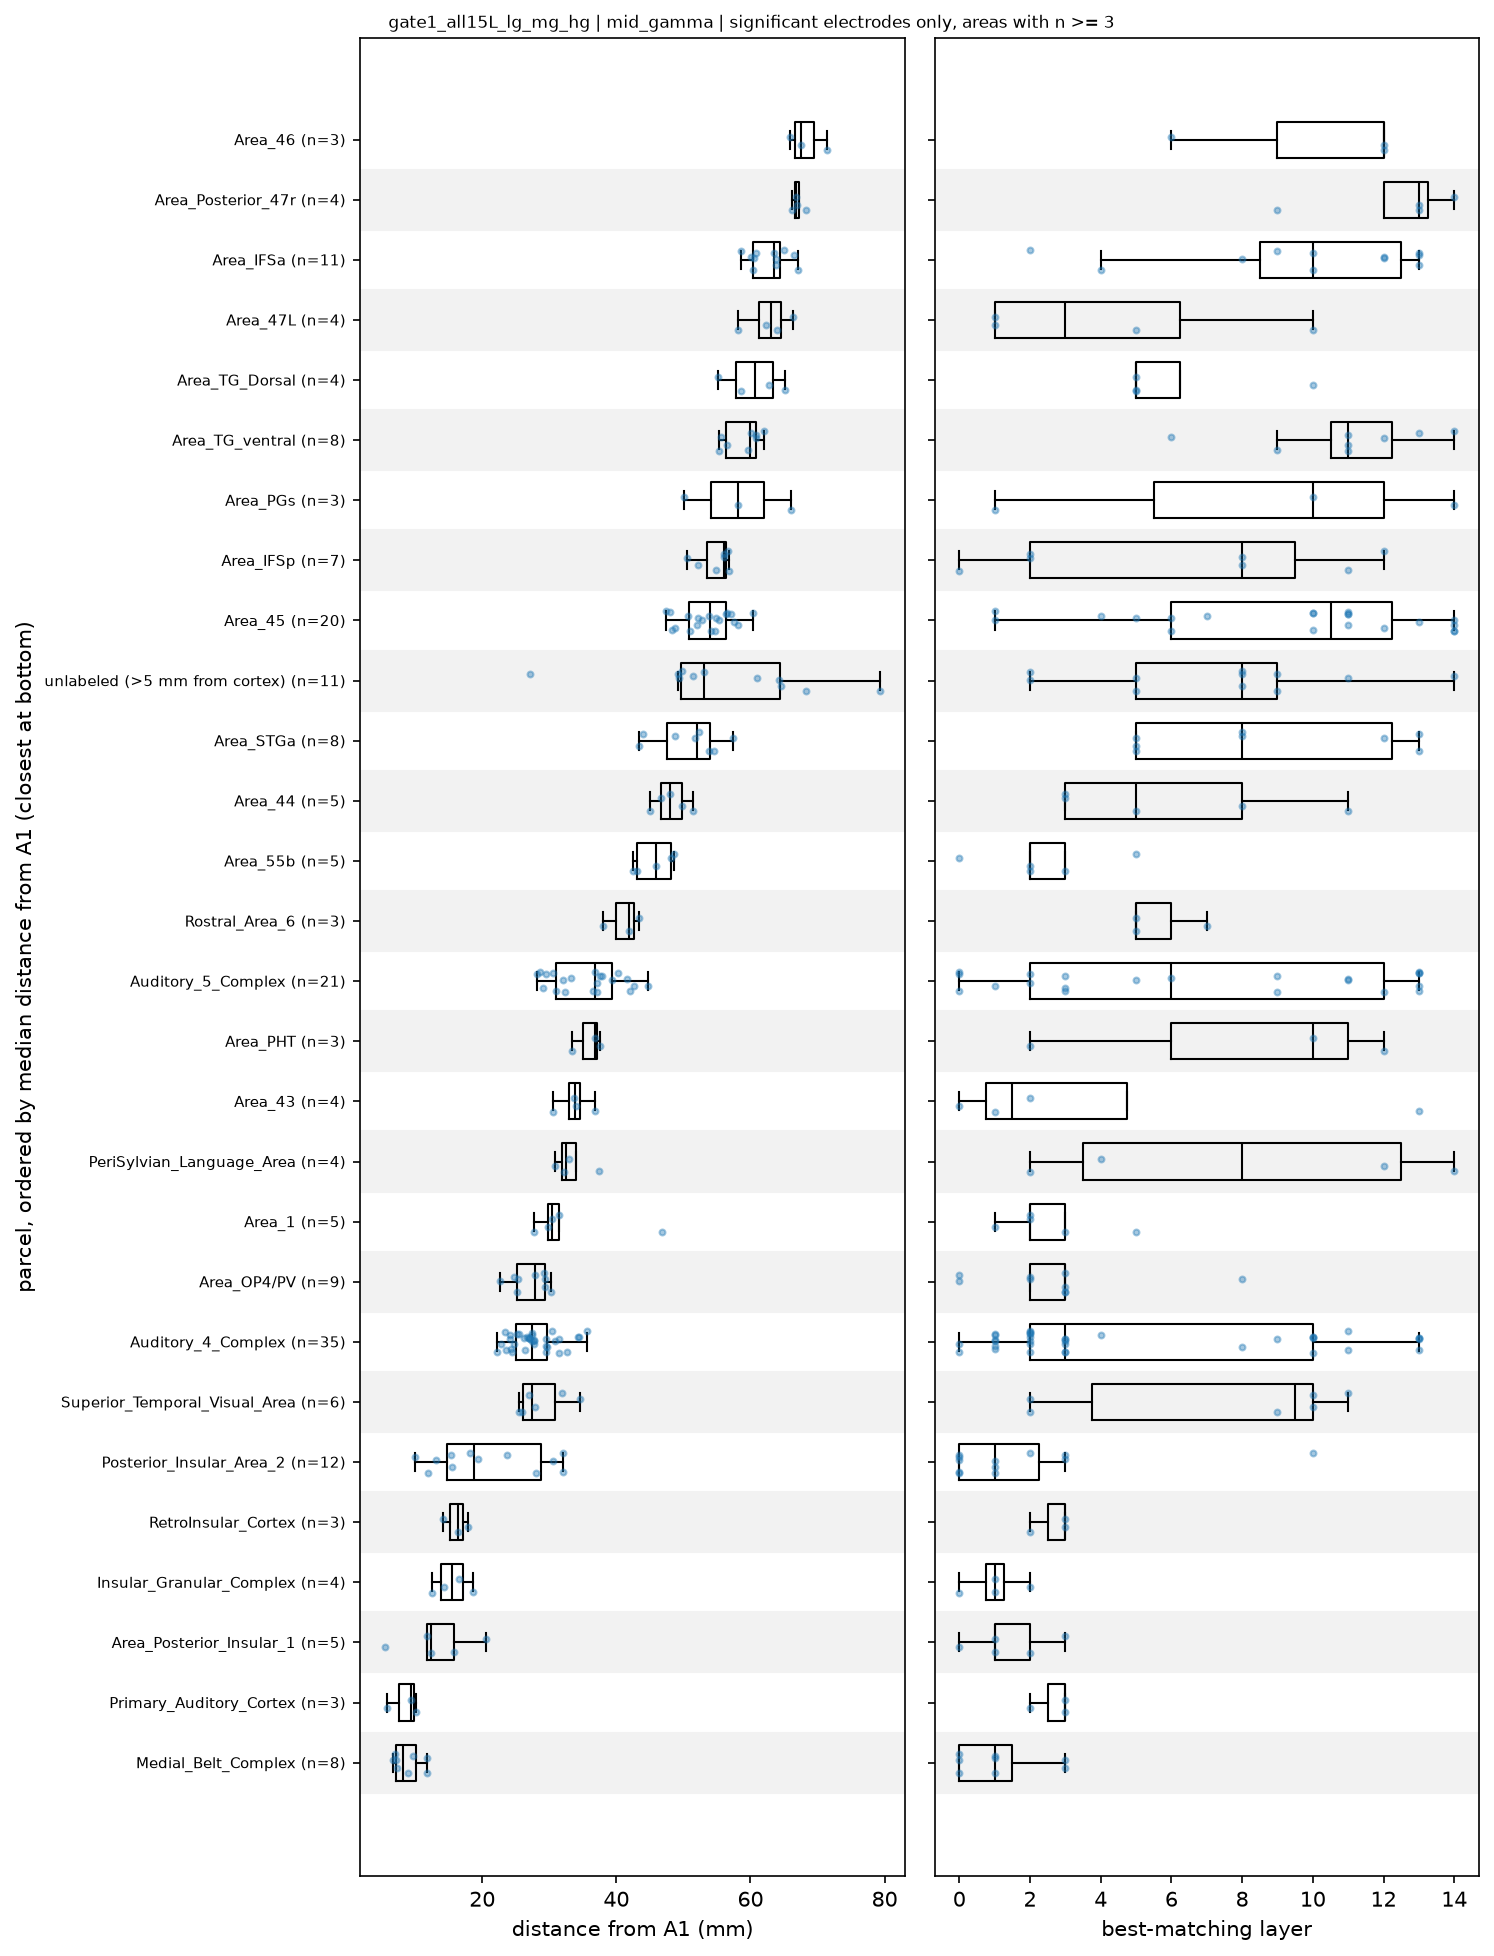
\includegraphics[width=\linewidth,height=0.82\textheight,keepaspectratio]{figures/areas_mid_gamma.png}
\caption{Mid-gamma best-matching layer by parcel, for parcels with at least 3 significant electrodes (218 of 260 electrodes). Layout as in Figure~\ref{fig:areas}.}
\end{figure}
\clearpage
\begin{figure}[H]
\centering
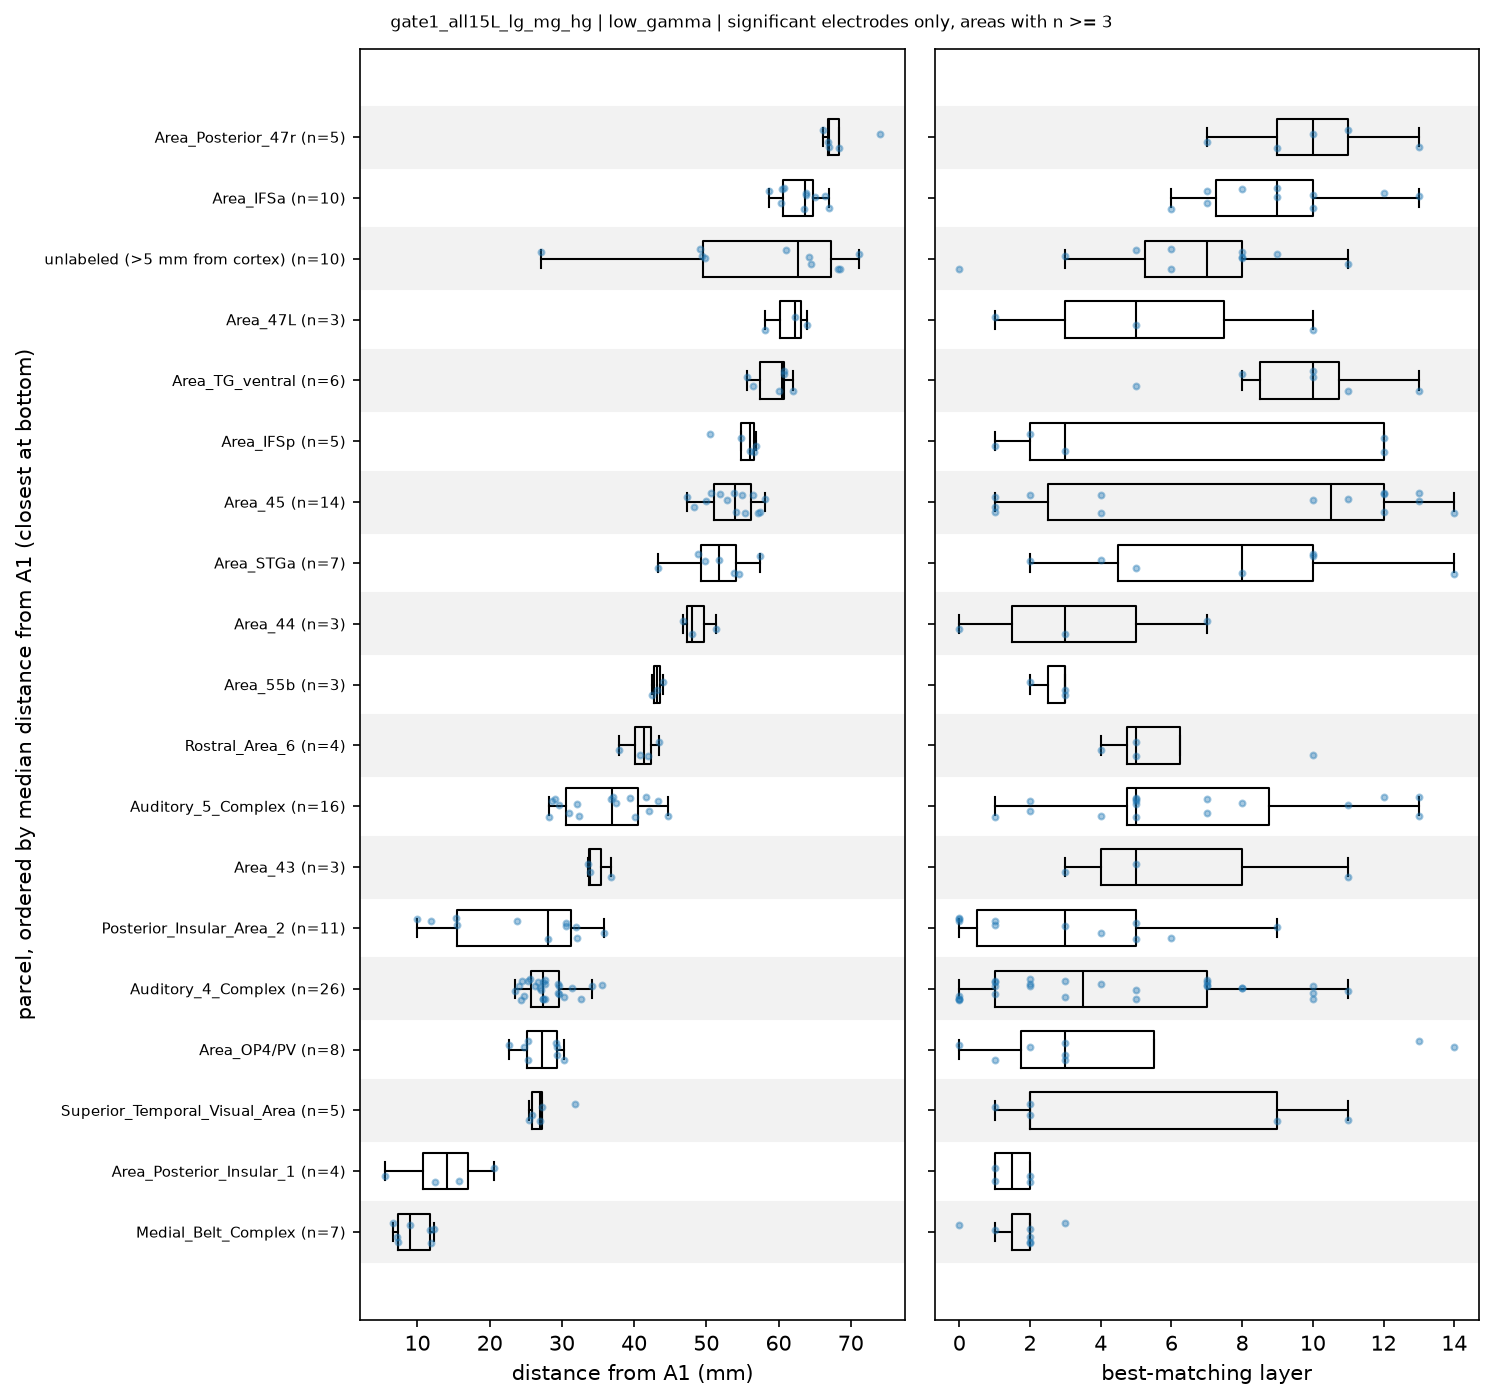
\includegraphics[width=\linewidth,height=0.82\textheight,keepaspectratio]{figures/areas_low_gamma.png}
\caption{Low-gamma best-matching layer by parcel, for parcels with at least 3 significant electrodes (150 of 191 electrodes). Layout as in Figure~\ref{fig:areas}.}
\end{figure}


\end{document}
